\documentclass[12pt]{article}
  \usepackage{geometry}
 \usepackage[round]{natbib}
 \usepackage{graphicx}
 \geometry{a4paper}
  \usepackage[T1]{fontenc}
  \usepackage[utf8]{inputenc}
  \usepackage{authblk}
  \usepackage[running]{lineno}
  \usepackage{setspace}
  \usepackage{booktabs}
  \usepackage{tabularx}
  \usepackage{chngpage}
  \usepackage{amsmath}
  \usepackage{amssymb}
  \usepackage[hidelinks]{hyperref}
 \usepackage[textsize=tiny]{todonotes}
\usepackage{pdfpages, caption}
\usepackage{listings}
\usepackage{framed}
\usepackage{mdframed}
\usepackage[section]{placeins}

\usepackage{natbib} %package for bibliography

\renewcommand{\thefigure}{S\arabic{figure}}
\renewcommand{\thetable}{S\arabic{table}}
\renewcommand{\thesection}{S\arabic{section}}


\newenvironment{problem}[2][Problem]{\begin{trivlist}
		\item[\hskip \labelsep {\bfseries #1}\hskip \labelsep {\bfseries #2.}]}{\end{trivlist}}

\DeclareMathOperator*{\argmax}{arg\,max}

\definecolor{apricot}{rgb}{0.984,0.81,0.69}
\BeforeBeginEnvironment{minted}{\begin{mdframed}[backgroundcolor=apricot]}
	\AfterEndEnvironment{minted}{\end{mdframed}}
\newcommand{\Lim}[1]{\raisebox{0.5ex}{\scalebox{0.8}{$\displaystyle \lim_{#1}\;$}}}
\newcommand*\widefbox[1]{\fbox{\hspace{2em}#1\hspace{2em}}}
\interfootnotelinepenalty=10000

\usepackage{framed}
\makeatletter
\newenvironment{kframe}{%
	\def\at@end@of@kframe{}%
	\ifinner\ifhmode%
	\def\at@end@of@kframe{\end{minipage}}%
\begin{minipage}{\columnwidth}%
	\fi\fi%
	\def\FrameCommand##1{\hskip\@totalleftmargin \hskip-\fboxsep
		\colorbox{shadecolor}{##1}\hskip-\fboxsep
		% There is no \\@totalrightmargin, so:
		\hskip-\linewidth \hskip-\@totalleftmargin \hskip\columnwidth}%
	\MakeFramed {\advance\hsize-\width
		\@totalleftmargin\z@ \linewidth\hsize
		\@setminipage}}%
{\par\unskip\endMakeFramed%
	\at@end@of@kframe}
\makeatother

\definecolor{fgcolor}{rgb}{0.345, 0.345, 0.345}
\newcommand{\hlnum}[1]{\textcolor[rgb]{0.686,0.059,0.569}{#1}}%
\newcommand{\hlstr}[1]{\textcolor[rgb]{0.192,0.494,0.8}{#1}}%
\newcommand{\hlcom}[1]{\textcolor[rgb]{0.678,0.584,0.686}{\textit{#1}}}%
\newcommand{\hlopt}[1]{\textcolor[rgb]{0,0,0}{#1}}%
\newcommand{\hlstd}[1]{\textcolor[rgb]{0.345,0.345,0.345}{#1}}%
\newcommand{\hlkwa}[1]{\textcolor[rgb]{0.161,0.373,0.58}{\textbf{#1}}}%
\newcommand{\hlkwb}[1]{\textcolor[rgb]{0.69,0.353,0.396}{#1}}%
\newcommand{\hlkwc}[1]{\textcolor[rgb]{0.333,0.667,0.333}{#1}}%
\newcommand{\hlkwd}[1]{\textcolor[rgb]{0.737,0.353,0.396}{\textbf{#1}}}%

\definecolor{orangeBright}{RGB}{243,146,0}
\definecolor{blueBright}{RGB}{54,169,225}
\definecolor{pinkBright}{RGB}{214,11,82}
\definecolor{shadecolor}{rgb}{.97, .97, .97}
\definecolor{messagecolor}{rgb}{0, 0, 0}
\definecolor{warningcolor}{rgb}{1, 0, 1}
\definecolor{errorcolor}{rgb}{1, 0, 0}
\newenvironment{knitrout}{}{} % an empty environment to be redefined in TeX


\usepackage{xr}
\externaldocument{figures}
\externaldocument{supplementary_materials_methods}

%   \doublespacing
% \raggedright
\title{Power analysis of MRR studies}
\author{Ben Lambert}

\begin{document}


\section{Power analysis of MRR studies}
Consider an ideal MRR experiment, where mosquitoes do not migrate out of the study area and marking is harmless. With these data, how accurately can we estimate mosquito lifespan? To address this question, we generated artificial MRR data and attempted to estimate the (known) parameters by maximum likelihood (a `Monte Carlo' analysis). We simulated releases of $N$ mosquitoes that are monitored for $m$ days in each case (with collections occurring on each day) and determined how the errors in estimating lifespan depended on these two parameters. In order to focus on estimating lifespan, we assumed the mosquitoes experience constant mortality, and recaptures follow the negative binomial sampling model where the (known) recapture probability parameters $\psi=0.03$ and $\kappa=3.18$ were the averages of the posterior draws across all species in the species-level model. We assume that all parameters: the true lifespan, $\psi$ and $\kappa$ were unknown and were estimated via maximum likelihood. Here, we investigated two lifespans: 5 days and 10 days indicative of estimates obtained in our analyses. For each simulation, we determined the Root Mean Square Error (RMSE) in predicting mean lifespan.

Unsurprisingly, the error in predicting lifespan declines as the study duration increases (Fig. \ref{fig:mrr_mcPowerAnalysis}A). However once a study length is much longer than the lifespan of the majority of mosquitoes, the predictive power cannot be improved by extending the study duration. The effect of increasing release size (while holding study length constant) similarly exhibits diminishing returns (Fig. \ref{fig:mrr_mcPowerAnalysis}B). For the parameters we use, there are significant gains in accuracy from releasing $1000$ rather than $100$ mosquitoes, but modest gains from releasing $10,000$ rather than $1000$ mosquitoes.

We also conducted a power analysis for the detection of senescence in MRR experiments (Fig. \ref{fig:mrr_mcPowerAnalysis_senescence}). Here we calculated the power to detect senescence assuming that lifespan follows a Gompertz survival function (see Table \ref{tab:mrr_survivalDescription}). We simulated MRR time series for single releases, for case study populations with three different levels of senescence assuming a Gompertz survival function (Fig. \ref{fig:mrr_mcPowerAnalysis_senescence}A.). We assumed that recaptures followed a negative binomial sampling model with $\psi=0.03$ and $\kappa=3.18$. Using each simulated time series of recaptures, we then performed two different maximum likelihood estimations: one, where we (falsely) assumed that lifespan followed an exponential distribution (i.e. there was no senescence); and another where we assumed it followed a Gompertz survival function. In both cases, we estimated the parameters of the corresponding survival function along with $\psi$ and $\kappa$. We then performed a likelihood ratio test (using a 5\% test size) comparing the fit of the Gompertz model to that of the simpler exponential model: in doing so, we determined whether there was evidence of senescence. We performed 500 experimental replicates at each parameter set.

These indicate that the power to detect senescence is strongly dependent on study length (Fig. \ref{fig:mrr_mcPowerAnalysis_senescence}B.) but is insensitive to release size (Fig. \ref{fig:mrr_mcPowerAnalysis_senescence}C.). \cite{clements1981analysis} conducted a meta-analysis of MRR and dissection-based experiments and found evidence of senescence that is, at least, qualitatively similar in magnitude to that of the `mild' case considered above. For this case, detecting senescence with a power of 80\% requires a study length of at least 18 days. Since the median study length for experiments included in our analysis was 10 days, (Table \ref{tab:mrr_aggregateData}) this could partly explain our failure to detect senescence at the species level.

\begin{figure}[ht]
	\centerline{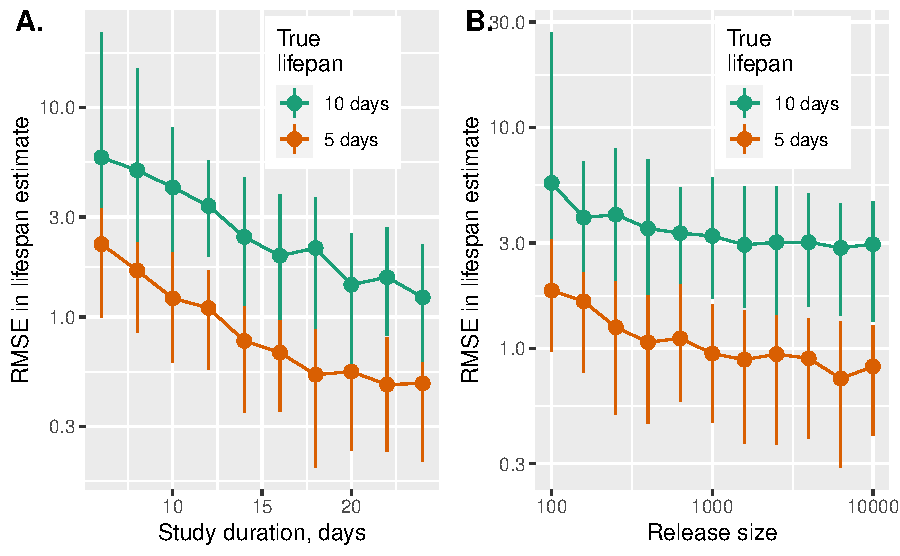
\includegraphics[width=1.25\textwidth]{./Figure_files/mrr_power_analysis.pdf}}
	\caption{\textbf{MRR: Monte Carlo analysis of errors in predicting mean lifespan.} This shows the Root Mean Square Error (RMSE) in predicting mean lifespan as a function of study length (A) and number of released mosquitoes (B) Monte Carlo analysis. For each parameter set, we generated 200 simulated data series using the negative binomial sampling model with an exponential survival function as described in the text and estimated the mean lifespan using maximum likelihood. The error bars show the 25\%-75\% quantiles, and the points show the medians.}
	\label{fig:mrr_mcPowerAnalysis}
\end{figure}

\begin{figure}[ht]
	\centerline{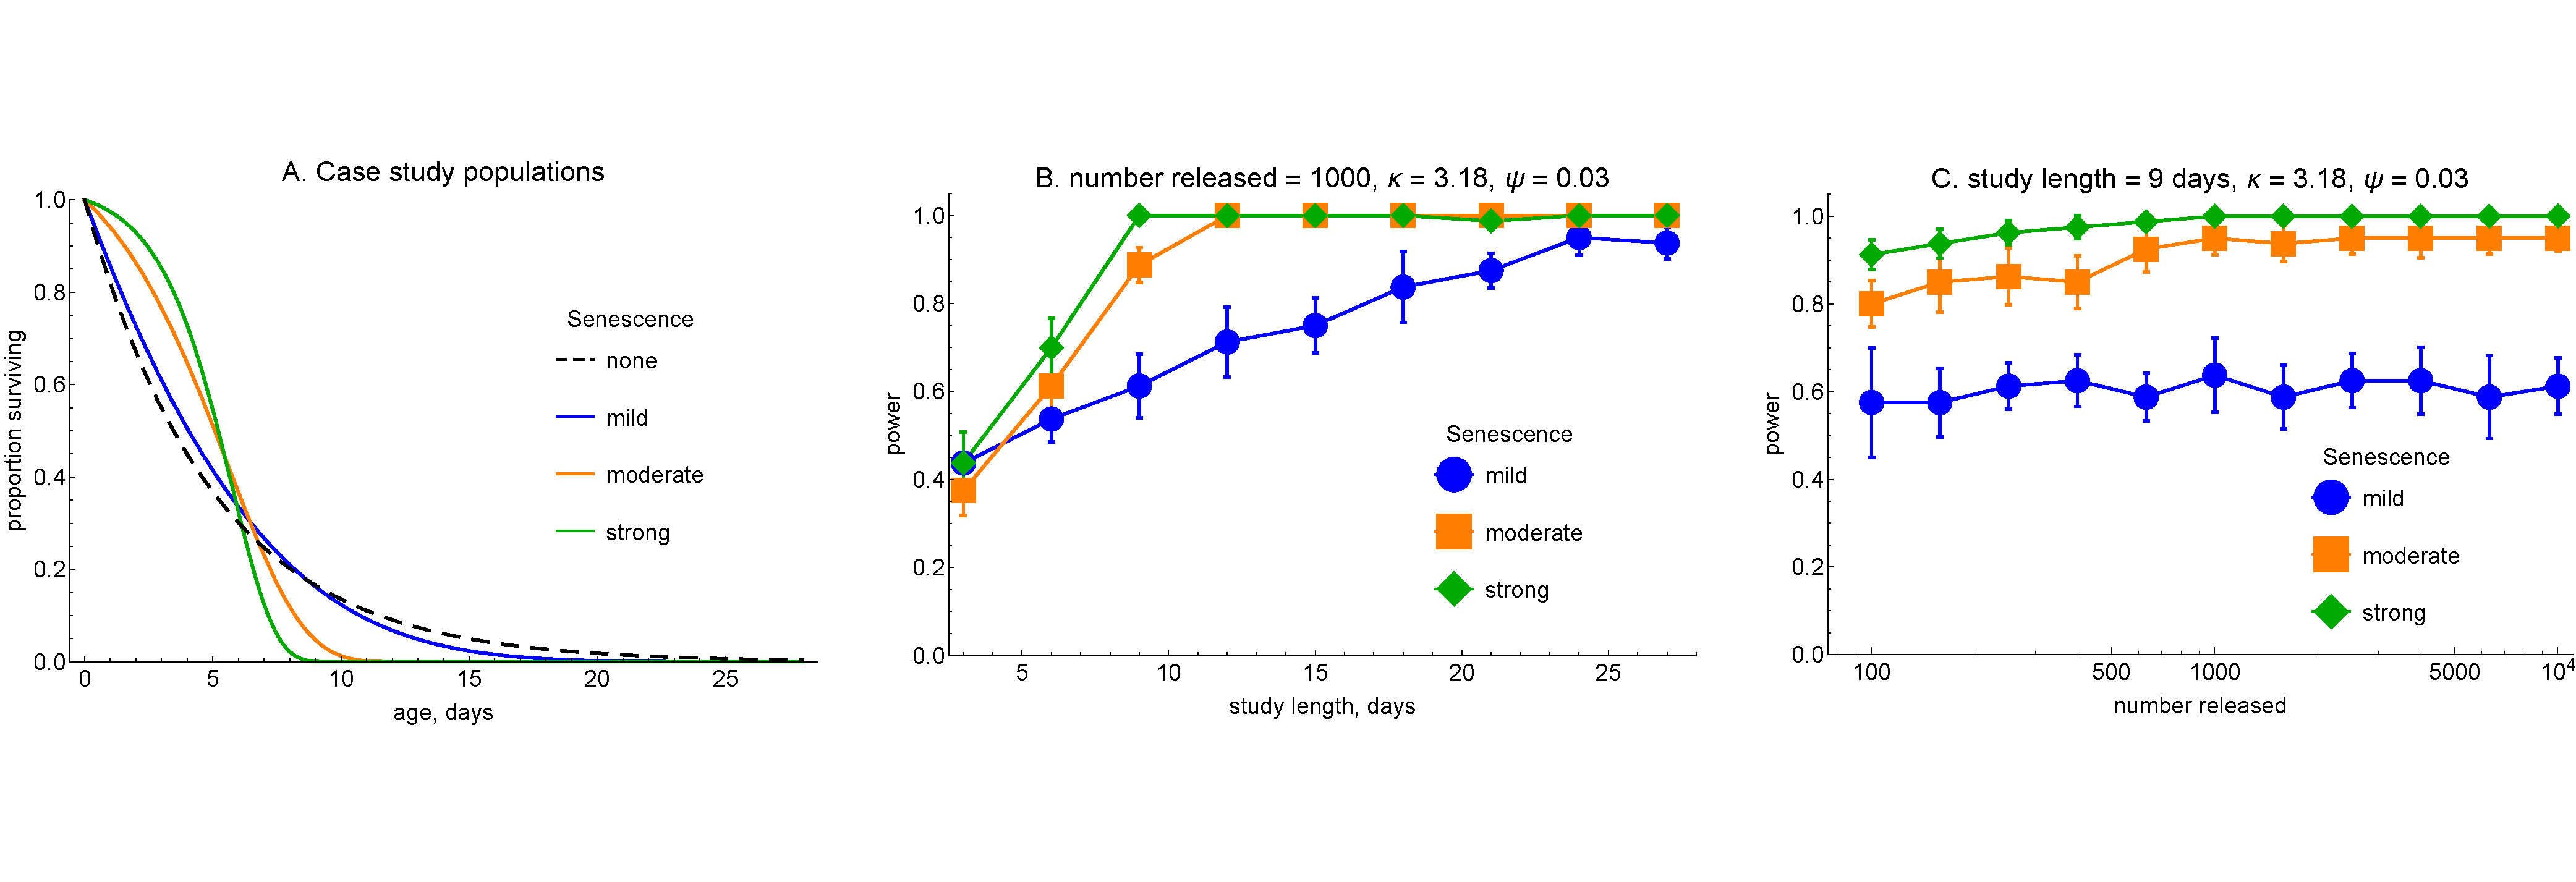
\includegraphics[width=1.25\textwidth]{./Figure_files/power-analysis-senescence.pdf}}
	\caption{\textbf{MRR: statistical power analysis for senescence detection.} The plot shows the statistical power to detect senescence for A. three case study populations as a function of B. study length and C. number released. For each parameter set we generated 500 simulated data series using the negative binomial sampling model with a gompertz hazard function ($\lambda(t) = \alpha e^{\beta t}$), and estimated the $\beta$ parameter using maximum likelihood and tested the null hypothesis $\beta=0$ (constant mortality risk) against the alternative $\beta>0$ using an likelihood ratio test with a 5\% test size. The error bars show the standard deviation in the power for each parameter set using groups of 40 simulated time series as bootstrap samples.}
	\label{fig:mrr_mcPowerAnalysis_senescence}
\end{figure}


\bibliographystyle{authordate1}
\bibliography{Malaria}

\end{document}